\documentclass[10pt]{article}
\usepackage[polish]{babel}
\usepackage[utf8]{inputenc}
\usepackage[T1]{fontenc}
\usepackage{graphicx}
\usepackage[export]{adjustbox}
\graphicspath{ {./images/} }
\usepackage{amsmath}
\usepackage{amsfonts}
\usepackage{amssymb}
\usepackage[version=4]{mhchem}
\usepackage{stmaryrd}
\usepackage{multirow}

\title{w Bydgoszczy }

\author{}
\date{}


\begin{document}
\maketitle
Kujawsko-Pomorskie Centrum Edukacji Nauczycieli

PLACÓWKA AKREDYTOWANA\\

\includegraphics[max width=\textwidth, center]{2024_11_21_997c30e0b98e62837d84g-01}

\section*{PESEL}
WEOCEAWEK

\section*{PRÓBNY EGZAMIN MATURALNY \\
 Z MATEMATYKI}
\section*{POZIOM PODSTAWOWY}
\begin{enumerate}
  \item Sprawdź, czy arkusz egzaminacyjny zawiera 18 stron (zadania 1-34). Ewentualny brak zgłoś przewodniczącemu zespołu nadzorującego próbny egzamin.
  \item Rozwiązania zadań i odpowiedzi wpisuj w miejscu na to przeznaczonym.
  \item Odpowiedzi do zadań zamkniętych (1-25) przenieś na kartę odpowiedzi, zaznaczając je w części karty przeznaczonej dla zdającego. Zamaluj ■ pola do tego przeznaczone. Błędne zaznaczenie otocz kółkiem i zaznacz właściwe.
  \item Pamiętaj, że pominięcie argumentacji lub istotnych obliczeń
\end{enumerate}

Marzec 2020

Czas pracy:\\
170 minut

Liczba punktów do uzyskania: 50\\
w rozwiązaniu zadania otwartego (26-34) może spowodować, że za to rozwiązanie nie będziesz mógł dostać pełnej liczby punktów.\\
5. Pisz czytelnie i używaj tylko długopisu lub pióra z czarnym tuszem lub atramentem.\\
6. Nie używaj korektora, a błędne zapisy wyraźnie przekreśl.\\
7. Pamiętaj, że zapisy w brudnopisie nie będą oceniane.\\
8. Możesz korzystać z zestawu wzorów matematycznych, cyrkla i linijki oraz kalkulatora.\\
9. Na karcie odpowiedzi wpisz swój numer PESEL.\\
10. Nie wpisuj żadnych znaków w części przeznaczonej dla egzaminatora.

\section*{ZADANIA ZAMKNIETE}
W zadaniach od 1. do 25. wybierz i zaznacz na karcie odpowiedzi poprawna odpowiedz.

\section*{Zadanie 1. (0-1 pkt)}
Zysk ze sprzedaży towaru w pewnej hurtowni w pierwszym miesiącu był równy 5000 zt , a w każdym następnym miesiącu o 5\% wyższy w stosunku do miesiąca poprzedniego. Zysk hurtowni w szóstym miesiącu jej działalności opisuje wzór\\
A. \(5000 \cdot 6 \cdot 1,05\)\\
B. \(5000 \cdot 1,05^{6}\)\\
C. \(5000 \cdot 5 \cdot 1,05\)\\
D. \(5000 \cdot 1,05^{5}\)

\section*{Zadanie 2.(0-1 pkt)}
Liczba \(2 \sqrt[5]{243}-\sqrt[3]{25} \cdot 3 \sqrt[3]{-5}+\sqrt[4]{256}\) jest równa\\
A. 25\\
B. 15\\
C. 12\\
D. -5

\section*{Zadanie 3. (0-1 pkt)}
Wartość wyrażenia \(\log _{2} 8 \sqrt{2}\) jest równa\\
A. \(\frac{3}{2}\)\\
B. \(\frac{5}{2}\)\\
C. \(\frac{7}{2}\)\\
D. \(\frac{9}{2}\)

\section*{Zadanie 4.(0-1 pkt)}
Wyrażenie \((x-3)^{2}-(x+1)(x-1)\) można przedstawić w postaci\\
A. 8\\
B. \(8-6 x\)\\
C. 10\\
D. \(10-6 x\)

\section*{Zadanie 5.(0-1 pkt)}
Najmniejszą liczbą całkowitą spełniającą nierówność \(\quad x-\frac{7 x-10}{4}<\frac{1}{2}\) jest liczba\\
A. -4\\
B. -3\\
C. 2\\
D. 3

\section*{Zadanie 6. (0-1 pkt)}
Równanie \(\left(\frac{1}{2} x-1,5\right)\left(x^{2}-16\right)=0\)\\
A. ma trzy różne rozwiązania\\
B. ma dwa różne rozwiązania\\
C. ma jedno rozwiązanie\\
D. nie ma rozwiązań.\\

\includegraphics[max width=\textwidth, center]{2024_11_21_997c30e0b98e62837d84g-03}

\section*{Zadanie 7. (0-1 pkt)}
Na rysunku poniżej przedstawiony jest wykres funkcji \(f\).\\
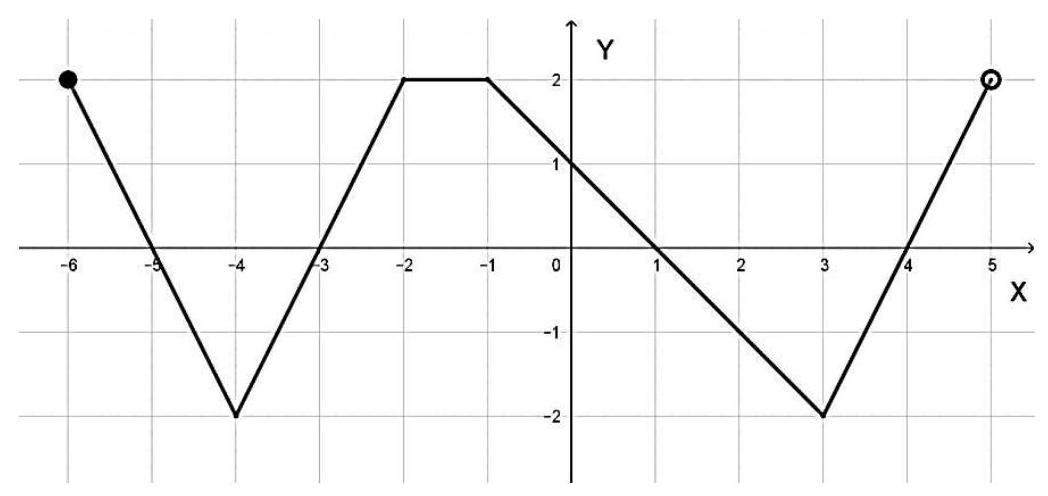
\includegraphics[max width=\textwidth, center]{2024_11_21_997c30e0b98e62837d84g-04}

Funkcja ta przyjmuje wartości nieujemne dla\\
A. \(x \in\langle-5,-3\rangle \cup\langle 1,4\rangle\)\\
B. \(x \in(-5,-3) \cup(1,4)\)\\
C. \(x \in\langle-6,-5) \cup(-3,1) \cup(4,5)\)\\
D. \(x \in\langle-6,-5\rangle \cup\langle-3,1\rangle \cup\langle 4,5)\)

\section*{Zadanie 8. (0-1 pkt)}
Wykres funkcji \(f\) przedstawionej na rysunku powstał przez przesunięcie wykresu funkcji \(g(x)=\frac{4}{x}\) wzdłuż osi odciętych. Funkcja \(f\) jest określona wzorem:\\
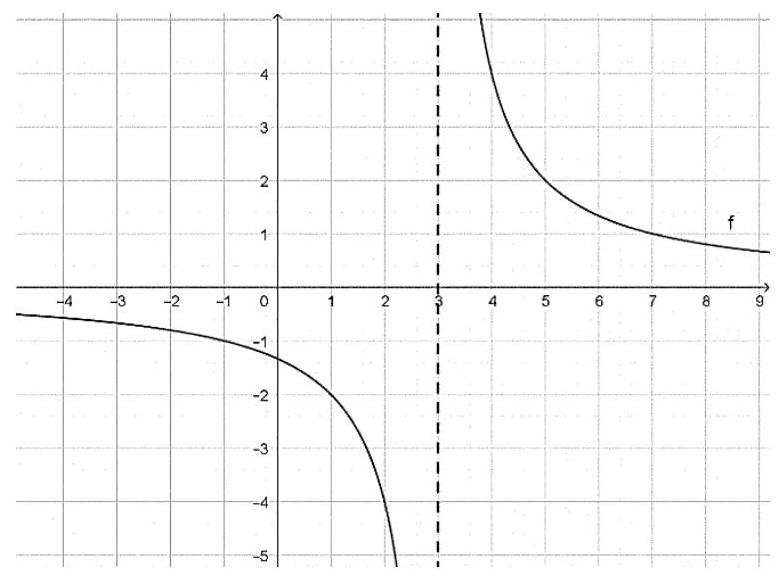
\includegraphics[max width=\textwidth, center]{2024_11_21_997c30e0b98e62837d84g-04(1)}\\
A. \(f(x)=\frac{4}{x+3}\)\\
B. \(f(x)=\frac{4}{x}-3\)\\
C. \(f(x)=\frac{4}{x-3}\)\\
D. \(f(x)=\frac{4}{x}+3\)

\section*{Zadanie 9. (0-1 pkt)}
Funkcja liniowa \(f(x)=-(m+1) x+m-1\) jest rosnąca dla\\
A. \(m>-1\)\\
B. \(m<-1\)\\
C. \(m>1\)\\
D. \(m<1\)

\section*{Zadanie 10.(0-1 pkt)}
Wykres funkcji liniowej \(f\) jest nachylony do osi \(O X\) pod kątem \(135^{\circ}\). Wiadomo, że \(f(-3)=8\). Funkcja liniowa \(f\) jest określona wzorem:\\
A. \(8 x+3 y=0\)\\
B. \(x+y-5=0\)\\
C. \(27 x-y+11=0\)\\
D. \(-3 x+8 y=0\)\\

\includegraphics[max width=\textwidth, center]{2024_11_21_997c30e0b98e62837d84g-05}

\section*{Zadanie 11. (0-1 pkt)}
Proste \(\mathrm{k}, \mathrm{l}, \mathrm{m}\) dane są równaniami \(k: y=\frac{3}{2}+\frac{2}{3} x, \quad l: y=-\frac{3}{2} x+\frac{1}{2}, \quad m: y=-\frac{2}{3} x+1\).\\
Wynika stąd, że\\
A. proste \(k i l\) są prostopadłe\\
B. proste \(k\) i \(m\) są prostopadłe\\
C. proste \(l\) i m są prostopadłe\\
D. wśród prostych \(k, l, m\) nie ma prostych prostopadłych

\section*{Zadanie 12. (0-1 pkt)}
Punkt \(A^{\prime}\) jest obrazem punktu \(A(-1 ;-2)\) w symetrii względem prostej \(x+4=0\). Zatem\\
A. \(A^{\prime}(-1 ; 9)\)\\
B. \(A^{\prime}(-7 ;-2)\)\\
C. \(A^{\prime}(-1 ;-6)\)\\
D. \(A^{\prime}(9 ;-2)\)

\section*{Zadanie 13. (0-1 pkt)}
Punkt \(W=(-1 ; 3)\) jest wierzchołkiem wykresu funkcji kwadratowej \(f\). Wobec tego funkcję \(f\) może przedstawiać wzór\\
A. \(f(x)=2(x-1)^{2}+3\)\\
B. \(f(x)=2(x-1)^{2}-3\)\\
C. \(f(x)=2(x+1)^{2}+3\)\\
D. \(f(x)=2(x+1)^{2}-3\)

\section*{Zadanie 14. (0-1 pkt)}
Dany jest ciąg \(a_{n}=\frac{n-15}{n}\). Liczba całkowitych wyrazów tego ciągu jest równa\\
A. 0\\
B. 1\\
C. 3\\
D. 4

\section*{Zadanie 15. (0-1 pkt)}
Liczby \(3, x^{3},-57\) tworzą w podanej kolejności ciąg arytmetyczny. Liczba \(x\) jest równa\\
A. -3\\
B. 3\\
C. \(\sqrt[3]{30}\)\\
D. \(\sqrt[3]{60}\)

\section*{Zadanie 16. (0-1 pkt)}
W rosnącym ciągu geometrycznym \(a_{1}=3\) oraz \(S_{3}=21\). Iloraz tego ciągu jest równy\\
A. -3\\
B. \(\frac{1}{2}\)\\
C. 2\\
D. 3\\

\includegraphics[max width=\textwidth, center]{2024_11_21_997c30e0b98e62837d84g-07}

\section*{Zadanie 17. (0-1 pkt)}
Liczba \(3 \cos ^{2} 67^{\circ}+2 \cos ^{2} 23^{\circ}+\sin ^{2} 67^{\circ}\) jest równa\\
A. 3\\
B. 1\\
C. \(\cos ^{2} 67^{\circ}\)\\
D. \(2 \sin ^{2} 23^{0}\)

\section*{Zadanie 18. (0-1 pkt)}
Dany jest trójkąt prostokątny o bokach długości \(a, b, c\).\\
Jeżeli \(\sin \alpha=0,28\) oraz \(a=7\), to\\
A. \(b=\sqrt{74}\)\\
B. \(b=25\)\\
C. \(b=24\)\\
D. \(b=\sqrt{774}\)\\
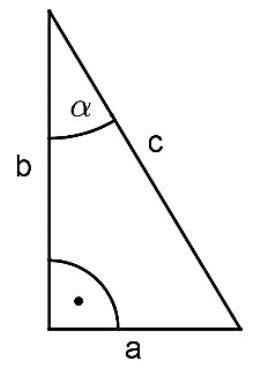
\includegraphics[max width=\textwidth, center]{2024_11_21_997c30e0b98e62837d84g-08(1)}

\section*{Zadanie 19. (0-1 pkt)}
Okręgi o promieniach 4 cm oraz 6 cm są styczne zewnętrznie. Prosta, która jest styczna do okręgu o promieniu 6 cm w punkcie \(K\) przechodzi przez środek okręgu o promieniu 4 cm (patrz rysunek). Długość odcinka \(K S_{1}\) jest równa\\
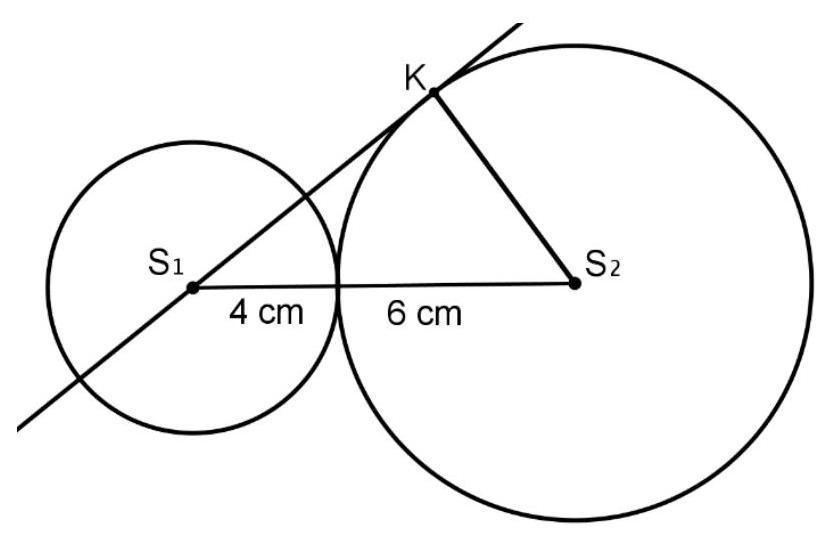
\includegraphics[max width=\textwidth, center]{2024_11_21_997c30e0b98e62837d84g-08(2)}\\
A. 6 cm\\
B. 8 cm\\
C. 10 cm\\
D. \(6 \sqrt{2} \mathrm{~cm}\)

\section*{Zadanie 20. (0-1 pkt)}
Pole rombu o boku 6 i kącie rozwartym \(150^{\circ}\) jest równe\\
A. \(18 \sqrt{2}\)\\
B. 18\\
C. \(36 \sqrt{2}\)\\
D. 36

\section*{Zadanie 21. (0-1 pkt)}
Punkt \(S\) jest środkiem okręgu. Miara kąta środkowego \(\alpha\) jest równa\\
A. \(36^{0}\)\\
B. \(72^{0}\)\\
C. \(120^{0}\)\\
D. \(144^{0}\)\\
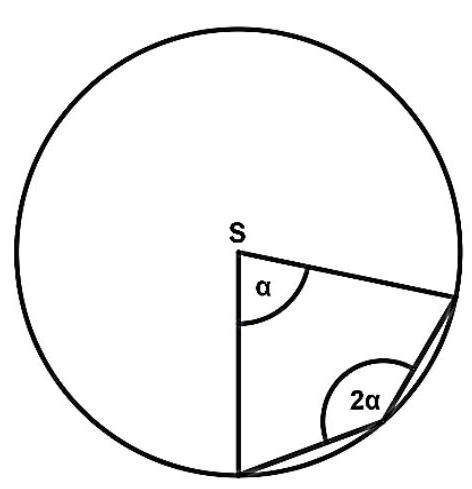
\includegraphics[max width=\textwidth, center]{2024_11_21_997c30e0b98e62837d84g-08}\\

\includegraphics[max width=\textwidth, center]{2024_11_21_997c30e0b98e62837d84g-09}

\section*{Zadanie 22. (0-1 pkt)}
Powierzchnia boczna stożka o promieniu podstawy 6 cm , po rozwinięciu jest wycinkiem koła o kącie \(120^{\circ}\). Pole powierzchni bocznej tego stożka jest równe\\
A. \(12 \pi\)\\
B. \(36 \pi\)\\
C. \(72 \pi\)\\
D. \(108 \pi\)

\section*{Zadanie 23. (0-1 pkt)}
Pewien graniastosłup ma 57 krawędzi. Liczba wszystkich ścian tego graniastosłupa jest równa\\
A. 19\\
B. 21\\
C. 38\\
D. 57

\section*{Zadanie 24. (0-1 pkt)}
Na diagramie przestawiono wzrost pięciorga uczniów. Odchylenie standardowe zestawu danych jest równe\\
A. 2 cm\\
B. \(\sqrt{2} \mathrm{~cm}\)\\
C. \(\sqrt{2,8} \mathrm{~cm}\)\\
D. \(2,8 \mathrm{~cm}\)

\section*{Zadanie 25.(0-1 pkt)}
Z cyfr 1, 2, 3, 4, 5, 6 tworzymy sześciocyfrowe liczby o niepowtarzających się cyfrach w taki sposób, że cyfry parzyste zapisane są obok siebie. Powstało w ten sposób\\
A. 36 liczb\\
B. 132 liczby\\
C. 144 liczby\\
D. 720 liczb\\

\includegraphics[max width=\textwidth, center]{2024_11_21_997c30e0b98e62837d84g-11}

\section*{ZADANIA OTWARTE}
Rozwiazania zadań o numerach od 26. do 34. należ̀y zapisać w wyznaczonych miejscach pod treścia zadania.

\section*{Zadanie 26. (0-2 pkt)}
Rozwiąż nierówność \(x^{2}+16 \geq 10 x+40\)\\

\includegraphics[max width=\textwidth, center]{2024_11_21_997c30e0b98e62837d84g-12}

\section*{Odpowiedź:}
\section*{Zadanie 27. (0-2 pkt)}
Udowodnij, że dla każdej liczby naturalnej \(n\), gdzie \(n \geq 1\), liczba \(2^{n}+2^{n+1}+2^{n+2}+2^{n+3}\) jest podzielna przez 30.

\begin{center}
\begin{tabular}{|c|c|c|c|c|c|c|c|c|c|c|c|c|c|c|c|c|c|c|c|c|c|c|}
\hline
 &  &  &  &  &  &  &  &  &  &  &  &  &  &  &  &  &  &  &  &  &  &  \\
\hline
 &  &  &  &  &  &  &  &  &  &  &  &  &  &  &  &  &  &  &  &  &  &  \\
\hline
 &  &  &  &  &  &  &  &  &  &  &  &  &  &  &  &  &  &  &  &  &  &  \\
\hline
 &  &  &  &  &  &  &  &  &  &  &  &  &  &  &  &  &  &  &  &  &  &  \\
\hline
 &  &  &  &  &  &  &  &  &  &  &  &  &  &  &  &  &  &  &  &  &  &  \\
\hline
 &  &  &  &  &  &  &  &  &  &  &  &  &  &  &  &  &  &  &  &  &  &  \\
\hline
 &  &  &  &  &  &  &  &  &  &  &  &  &  &  &  &  &  &  &  &  &  &  \\
\hline
 &  &  &  &  &  &  &  &  &  &  &  &  &  &  &  &  &  &  &  &  &  &  \\
\hline
 &  &  &  &  &  &  &  &  &  &  &  &  &  &  &  &  &  &  &  &  &  &  \\
\hline
 &  &  &  &  &  &  &  &  &  &  &  &  &  &  &  &  &  &  &  &  &  &  \\
\hline
 &  &  &  &  &  &  &  &  &  &  &  &  &  &  &  &  &  &  &  &  &  &  \\
\hline
 &  &  &  &  &  &  &  &  &  &  &  &  &  &  &  &  &  &  &  &  &  &  \\
\hline
 &  &  &  &  &  &  &  &  &  &  &  &  &  &  &  &  &  &  &  &  &  &  \\
\hline
 &  &  &  &  &  &  &  &  &  &  &  &  &  &  &  &  &  &  &  &  &  &  \\
\hline
 &  &  &  &  &  &  &  &  &  &  &  &  &  &  &  & - &  &  &  &  &  &  \\
\hline
 &  &  &  &  &  &  &  &  &  &  &  &  &  &  &  &  &  &  &  &  &  &  \\
\hline
\end{tabular}
\end{center}

\section*{Zadanie 28. (0-2 pkt)}
Liczebność kolonii bakterii pewnego szczepu w zależności od czasu opisuje funkcja \(f(t)=m_{0} \cdot a^{t}\), gdzie \(\mathrm{t}-\) oznacza czas obserwacji w godzinach, \(a-\) pewną stałą dodatnią, a \(m_{0}\) - liczebność początkowej próby bakterii. Na początku doświadczenia zaobserwowano 300 sztuk bakterii. Po dwóch godzinach liczba bakterii wzrosła do 1200. Po jakim czasie liczba bakterii wzrośnie do 153600?\\

\includegraphics[max width=\textwidth, center]{2024_11_21_997c30e0b98e62837d84g-13}

Odpowiedź:

\section*{Zadanie 29. (0-2 pkt)}
Pole kwadratu \(A B C D\) jest równe 16. Punkt \(E\) jest środkiem boku \(B C\), a punkt \(S\) punktem przecięcia przekątnej \(B D\) kwadratu i odcinka \(A E\). Wykaż, że odległość punktu \(S\) od boku \(A B\) jest równa \(\frac{4}{3}\).\\

\includegraphics[max width=\textwidth, center]{2024_11_21_997c30e0b98e62837d84g-14}

\section*{Zadanie 30. (0-2 pkt)}
Na sześciu jednakowych kartkach napisano liczby: 1, 10, 100, 1000, 10000, 100000. Z tych kartek losujemy kolejno bez zwracania trzy. Oblicz prawdopodobieństwo, że suma wylosowanych liczb tworzy liczbę podzielną przez cztery.

\begin{center}
\begin{tabular}{|c|c|c|c|c|c|c|c|c|c|c|c|c|c|c|c|c|c|c|c|c|c|c|c|c|c|c|c|c|c|c|c|}
\hline
 &  &  &  &  &  &  &  &  &  &  &  &  &  &  &  &  &  &  &  &  &  &  &  &  &  &  &  &  &  &  &  \\
\hline
 &  &  &  &  &  &  &  &  &  &  &  &  &  &  &  &  &  &  &  &  &  &  &  &  &  &  &  &  &  &  &  \\
\hline
 &  &  &  &  &  &  &  &  &  &  &  &  &  &  &  &  &  &  &  &  &  &  &  &  &  &  &  &  &  &  &  \\
\hline
 &  &  &  &  &  &  &  &  &  &  &  &  &  &  &  &  &  &  &  &  &  &  &  &  &  &  &  &  &  &  &  \\
\hline
 &  &  &  &  &  &  &  &  &  &  &  &  &  &  &  &  &  &  &  &  &  &  &  &  &  &  &  &  &  &  &  \\
\hline
 &  &  &  &  &  &  &  &  &  &  &  &  &  &  &  &  &  &  &  &  &  &  &  &  &  &  &  &  &  &  &  \\
\hline
 &  &  &  &  &  &  &  &  &  &  &  &  &  &  &  &  &  &  &  &  &  &  &  &  &  &  &  &  &  &  &  \\
\hline
 &  &  &  &  &  &  &  &  &  &  &  &  &  &  &  &  &  &  &  &  &  &  &  &  &  &  &  &  &  &  &  \\
\hline
 &  &  &  &  &  &  &  &  &  &  &  &  &  &  &  &  &  &  &  &  &  &  &  &  &  &  &  &  &  &  &  \\
\hline
 &  &  &  &  &  &  &  &  &  &  &  &  &  &  &  &  &  &  &  &  &  &  &  &  &  &  &  &  &  &  &  \\
\hline
 &  &  &  &  &  &  &  &  &  &  &  &  &  &  &  &  &  &  &  &  &  &  &  &  &  &  &  &  &  &  &  \\
\hline
 &  &  &  &  &  &  &  &  &  &  &  &  &  &  &  &  &  &  &  &  &  &  &  &  &  &  &  &  &  &  &  \\
\hline
 &  &  &  &  &  &  &  &  &  &  &  &  &  &  &  &  &  &  &  &  &  &  &  &  &  &  &  &  &  &  &  \\
\hline
 &  &  &  &  &  &  &  &  &  &  &  &  &  &  &  &  &  &  &  &  &  &  &  &  &  &  &  &  &  &  &  \\
\hline
 &  &  &  &  &  &  &  &  &  &  &  &  &  &  &  &  &  &  &  &  &  &  &  &  &  &  &  &  &  &  &  \\
\hline
\end{tabular}
\end{center}

Odpowiedź:\\
Zadanie 31. (0-2 pkt)\\
W ciągu arytmetycznym \(\left(a_{n}\right)\), dla \(n \geq 1\) suma wyrazów trzeciego, czwartego i piątego wynosi 144 . Oblicz sumę siedmiu kolejnych wyrazów ciągu \(\left(a_{n}\right)\).

\begin{center}
\begin{tabular}{|c|c|c|c|c|c|c|c|c|c|c|c|c|c|c|c|c|c|c|c|c|c|c|c|c|c|c|c|c|}
\hline
 &  &  &  &  &  &  &  &  &  &  &  &  &  &  &  &  &  &  &  &  &  &  &  &  &  &  &  &  \\
\hline
 &  &  &  &  &  &  &  &  &  &  &  &  &  &  &  &  &  &  &  &  &  &  &  &  &  &  &  &  \\
\hline
 &  &  &  &  &  &  &  &  &  &  &  &  &  &  &  &  &  &  &  &  &  &  &  &  &  &  &  &  \\
\hline
 &  &  &  &  &  &  &  &  &  &  &  &  &  &  &  &  &  &  &  &  &  &  &  &  &  &  &  &  \\
\hline
 &  &  &  &  &  &  &  &  &  &  &  &  &  &  &  &  &  &  &  &  &  &  &  &  &  &  &  &  \\
\hline
 &  &  &  &  &  &  &  &  &  &  &  &  &  &  &  &  &  &  &  &  &  &  &  &  &  &  &  &  \\
\hline
 &  &  &  &  &  &  &  &  &  &  &  &  &  &  &  &  &  &  &  &  &  &  &  &  &  &  &  &  \\
\hline
 &  &  &  &  &  &  &  &  &  &  &  &  &  &  &  &  &  &  &  &  &  &  &  &  &  &  &  &  \\
\hline
 &  &  &  &  &  &  &  &  &  &  &  &  &  &  &  &  &  &  &  &  &  &  &  &  &  &  &  &  \\
\hline
 &  &  &  &  &  &  &  &  &  &  &  &  &  &  &  &  &  &  &  &  &  &  &  &  &  &  &  &  \\
\hline
 &  &  &  &  &  &  &  &  &  &  &  &  &  &  &  &  &  &  &  &  &  &  &  &  &  &  &  &  \\
\hline
 &  &  &  &  &  &  &  &  &  &  &  &  &  &  &  &  &  &  &  &  &  &  &  &  &  &  &  &  \\
\hline
 &  &  &  &  &  &  &  &  &  &  &  &  &  &  &  &  &  &  &  &  &  &  &  &  &  &  &  &  \\
\hline
 &  &  &  &  &  &  &  &  &  &  &  &  &  &  &  &  &  &  &  &  &  &  &  &  &  &  &  &  \\
\hline
 &  &  &  &  &  &  &  &  &  &  &  &  &  &  &  &  &  &  &  &  &  &  &  &  &  &  &  &  \\
\hline
 &  &  &  &  &  &  &  &  &  &  &  &  &  &  &  &  &  &  &  &  &  &  &  &  &  & 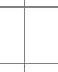
\includegraphics[max width=\textwidth]{2024_11_21_997c30e0b98e62837d84g-15}
 &  &  \\
\hline
 &  &  &  &  &  &  &  &  &  &  &  &  &  &  &  &  &  &  &  &  &  &  &  &  &  & \( 1 \) &  &  \\
\hline
\end{tabular}
\end{center}

Odpowiedź:

\section*{Zadanie 32. (0 - 4 pkt)}
W trójkącie rozwartokątnym \(A B C\) o kącie rozwartym przy wierzchołku \(C\) poprowadzono wysokość \(C D\) i otrzymano równoramienny trójkąt \(A C D\). Długości boków \(A B\) i \(A C\) są odpowiednio równe \(|A B|=4(1+\sqrt{3})\) i \(|A C|=4 \sqrt{2}\). Oblicz pole powierzchni koła opisanego na trójkącie \(A B C\).\\

\includegraphics[max width=\textwidth, center]{2024_11_21_997c30e0b98e62837d84g-16}\\

\includegraphics[max width=\textwidth, center]{2024_11_21_997c30e0b98e62837d84g-17}

Odpowiedź:

\section*{Zadanie 33. (0 - 4 pkt)}
Właściciel sklepu kupuje zegarki płacąc producentowi \(180 \mathrm{zł}\) za sztukę. Następnie sprzedaje miesięcznie 30 sztuk takich zegarków po 230 zł. Sprzedawca oszacował, że każda obniżka ceny zegarka o złotówkę zwiększy liczbę sprzedanych zegarków o trzy sztuki. Niech \(x\) oznacza liczbę obniżek o 1zł, gdzie \(x \in\{1,2,3, \ldots, 30\}\). Jaką powinien ustalić cenę, aby jego miesięczny zysk był największy?\\

\includegraphics[max width=\textwidth, center]{2024_11_21_997c30e0b98e62837d84g-18}

Odpowiedź:

\section*{Zadanie 34. (0 - 5 pkt)}
Pole podstawy ostrosłupa prawidłowego trójkątnego jest równe \(16 \sqrt{3}\), a jego objętość \(80 \sqrt{3}\). Wyznacz cosinus kąta \(\alpha\) nachylenia ściany bocznej do płaszczyzny podstawy.\\
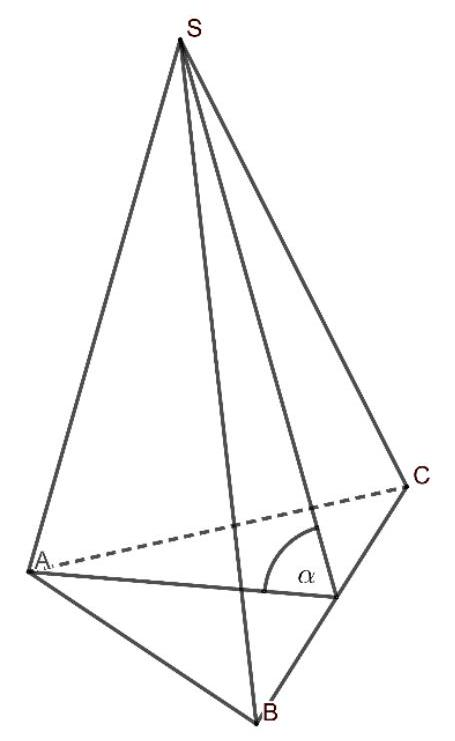
\includegraphics[max width=\textwidth, center]{2024_11_21_997c30e0b98e62837d84g-19}\\

\includegraphics[max width=\textwidth, center]{2024_11_21_997c30e0b98e62837d84g-19(1)}

Odpowiedź:

\section*{KOD}
\begin{center}
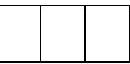
\includegraphics[max width=\textwidth]{2024_11_21_997c30e0b98e62837d84g-20}
\end{center}

\section*{PESEL}
\begin{center}
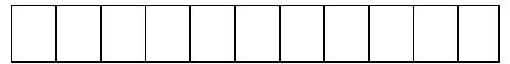
\includegraphics[max width=\textwidth]{2024_11_21_997c30e0b98e62837d84g-20(1)}
\end{center}

WYPELNIA ZDAJĄCY

\begin{center}
\begin{tabular}{|c|c|c|c|c|}
\hline
\multirow{2}{*}{\(
\begin{gathered}
\mathrm{Nr} \\
\mathrm{zad} .
\end{gathered}
\)} & \multicolumn{4}{|c|}{Odpowiedzi} \\
\hline
 & A & B & C & D \\
\hline
1 & ㅁ & ㅁ & ㅁ & ㅁ \\
\hline
2 & - & ㅁ & - & ㅁ \\
\hline
3 & ㅁ & ㅁ & ㅁ & ㅁ \\
\hline
4 & ㅁ & ㅁ & ㅁ & ㅁ \\
\hline
5 & ㅁ & ㅁ & ㅁ & ㅁ \\
\hline
6 & - & ㅁ & ㅁ & ㅁ \\
\hline
7 & ㅁ & ㅁ & ㅁ & ㅁ \\
\hline
8 & ㅁ & ㅁ & - & ㅁ \\
\hline
9 & - & ㅁ & ㅁ & ㅁ \\
\hline
10 & ㅁ & ㅁ & - & ㅁ \\
\hline
11 & ㅁ & ㅁ & ㅁ & ㅁ \\
\hline
12 & ㅁ & ㅁ & ㅁ & ㅁ \\
\hline
13 & ㅁ & ㅁ & ㅁ & ㅁ \\
\hline
14 & - & ㅁ & - & ㅁ \\
\hline
15 & - & ㅁ & - & - \\
\hline
16 & - & ㅁ & ㅁ & ㅁ \\
\hline
17 & ㅁ & ㅁ & ㅁ & ㅁ \\
\hline
18 & ㅁ & ㅁ & - & ㅁ \\
\hline
19 & ㅁ & ㅁ & - & ㅁ \\
\hline
20 & ㅁ & ㅁ & ㅁ & ㅁ \\
\hline
21 & - & ㅁ & ㅁ & ㅁ \\
\hline
22 & ㅁ & ㅁ & ㅁ & ㅁ \\
\hline
23 & - & ㅁ & ㅁ & ㅁ \\
\hline
24 & ㅁ & ㅁ & ㅁ & ㅁ \\
\hline
25 & ㅁ & ㅁ & ㅁ & ㅁ \\
\hline
\end{tabular}
\end{center}

WYPELNIA EGZAMINATOR

\begin{center}
\begin{tabular}{|c|c|c|c|c|c|c|}
\hline
Nr & \multicolumn{6}{|c|}{Punkty} \\
\hline
zad. & \(\mathbf{0}\) & \(\mathbf{1}\) & \(\mathbf{2}\) & \(\mathbf{3}\) & \(\mathbf{4}\) & \(\mathbf{5}\) \\
\hline
\(\mathbf{2 6}\) & \(\square\) & \(\square\) & \(\square\) &  &  &  \\
\hline
\(\mathbf{2 7}\) & \(\square\) & \(\square\) & \(\square\) &  &  &  \\
\hline
\(\mathbf{2 8}\) & \(\square\) & \(\square\) & \(\square\) &  &  &  \\
\hline
\(\mathbf{2 9}\) & \(\square\) & \(\square\) & \(\square\) &  &  &  \\
\hline
\(\mathbf{3 0}\) & \(\square\) & \(\square\) & \(\square\) &  &  &  \\
\hline
\(\mathbf{3 1}\) & \(\square\) & \(\square\) & \(\square\) &  &  &  \\
\hline
\(\mathbf{3 2}\) & \(\square\) & \(\square\) & \(\square\) & \(\square\) & \(\square\) &  \\
\hline
\(\mathbf{3 3}\) & \(\square\) & \(\square\) & \(\square\) & \(\square\) & \(\square\) &  \\
\hline
\(\mathbf{3 4}\) & \(\square\) & \(\square\) & \(\square\) & \(\square\) & \(\square\) & \(\square\) \\
\hline
\end{tabular}
\end{center}

SUMA PUNKTÓW


\end{document}